\chapter{Linear Regression}
A major component of machine learning, the one that most people associate with ML, is dedicated to making predictions under uncertain conditions. Given some input data, we would like to produce a target output. In this chapter, we're going to focus on the case where our prediction is a continuous, real number. This type of problem is known as \textbf{regression}.

\section{Introduction and Motivation}
We can imagine many situations where regression is useful:
\begin{enumerate}
    \item Predicting a person's height given the height of their parents.
    \item Predicting the probability that someone pays back a loan given their credit history.
    \item Predicting what time a package will arrive given current weather and traffic conditions.
\end{enumerate}

We're specifically going to focus on \textbf{linear regression}, which means that our goal is to find some linear combination of the $x_{1}, ..., x_{D}$ values that predict our target $y$.

\begin{definition}{Linear Regression}{linear-regression}
Suppose we have an input $\textbf{x}\in\mathbb{R}^D$ and a continuous target $y\in\mathbb{R}$.
Linear regression determines weights $w_{i}\in\mathbb{R}$ that balance the values of $x_{i}$ to produce $y$:
\begin{equation}
    y = w_{0} + w_{1}x_{1} + ... + w_{D}x_{D}
\end{equation}

\end{definition}

\readernote{Notice $w_{0}$ in the expression above, which doesn't have a corresponding $x_{0}$ value. This is known as the \textit{bias} term. If you consider the definition of a line $y = mx + b$, the bias term is comparable to the intercept $b$. It can account for a general trend in our data, such as if all of our target $y$ values are greater than 50.}

All of these follow a similar formula: a data input $\textbf{x}$ gets transformed into prediction $y$. For example, consider 10 year old Sam. She is curious about how tall she will be when she grows up. She has a data set of parents' heights and the final heights of their children. The inputs \textbf{x} are:

\begin{align*}
x_{1} = \text{height of mother (cm)} \\
x_{2} = \text{height of father (cm)} \\
\end{align*}

Using linear regression, she determines the weights \textbf{w} to be:

\begin{align*}
\textbf{w} = [34, 0.39, 0.33] \\
\end{align*}

Sam's mother is 165 cm tall and her father is 185 cm tall. Using the results of the linear regression solution, Sam solves for her expected height:

\begin{align*}
\text{Sam's height} = 34 + 0.39(165) + 0.33(185) = \textbf{159.4 cm} \\
\end{align*}

\begin{mlcube}{Linear Regression}
Let's inspect the categories linear regression falls into for our ML framework cube. First, as we've already stated, linear regression deals with a \textbf{continuous} input and output domain. Second, our goal is to make predictions on future data points, and to construct something capable of making those predictions we first need a labeled data set of inputs and outputs. This makes linear regression is a \textbf{supervised} technique. Third and finally, linear regression is a special case when it comes to being \textbf{probabilistic or non-probabilistic}. Depending on our interpretation, it can be either one! We will explain how this works later in the chapter.
\begin{center}
    \begin{tabular}{c|c|c}
    \textit{\textbf{Domain}} & \textit{\textbf{Training}} & \textit{\textbf{Probabilistic}} \\
    \hline
    Continuous & Supervised & Yes / No \\
    \end{tabular}
\end{center}
\end{mlcube}

\section{Technical}
The most basic form of linear regression is a simple weighted combination of the input variables $\textbf{x}$, which you will often see written as:

\begin{equation}
    y(\textbf{x}, \textbf{w}) = w_{0} + w_{1}x_{1} + ... + w_{D}x_{D}
\end{equation}

\subsubsection{Merging of Bias}
We're going to introduce a common notational trick here for making the bias term, $w_{0}$, easier to handle. At the moment $w_{0}$ is unwieldly because it is not being multiplied by an $x_{i}$ value. Without the bias term, we could easily express $y(\textbf{x}, \textbf{w})$ as:

\begin{equation}
    y(\textbf{x}, \textbf{w}) = \textbf{w}^{T}\textbf{x} = w_{0}x_{0} + w_{1}x_{1} + ... + w_{D}x_{D}
\end{equation}

 This is more compact, easier to reason about, and makes properties of linear algebra nicer for the calculations we will be performing. An easy way to keep our bias term and still get this nice form of $\textbf{w}^{T}\textbf{x}$ is to simply introduce another variable, $x_{0}$, that is always $1$ for every data point. For example, considering the case of Sam's height from above, we have the height of her parents, \textbf{x}:

\begin{align*}
    \textbf{x} = (165, 185)
\end{align*}

We now add a $1$ in the first position of the data point to make it:

\begin{align*}
    \textbf{x'} = (1, 165, 185)
\end{align*}

We do this for every point in our data set. This bias trick lets us write:

\begin{equation}
    y(\textbf{x}, \textbf{w}) = \textbf{w}^{T}\textbf{x} = w_{0}x_{0} + w_{1}x_{1} + ... + w_{D}x_{D}
\end{equation}

as desired.

\subsubsection{Visualization of Linear Regression}
Let's try to build some intuition about how linear regression works. Our algorithm is provided with a collection of data points: inputs \textbf{x} and corresponding targets \textbf{y}. Our goal is to find the best set of weights \textbf{w} such that given a new data point \textbf{x}, we can accurately predict the true target value $y$. This is visualizable in the simple case where $\textbf{x}$ is a 1-dimensional input variable, as in Figure \ref{fig:simple-lin-reg}:

\begin{figure}[H]
    \centering
    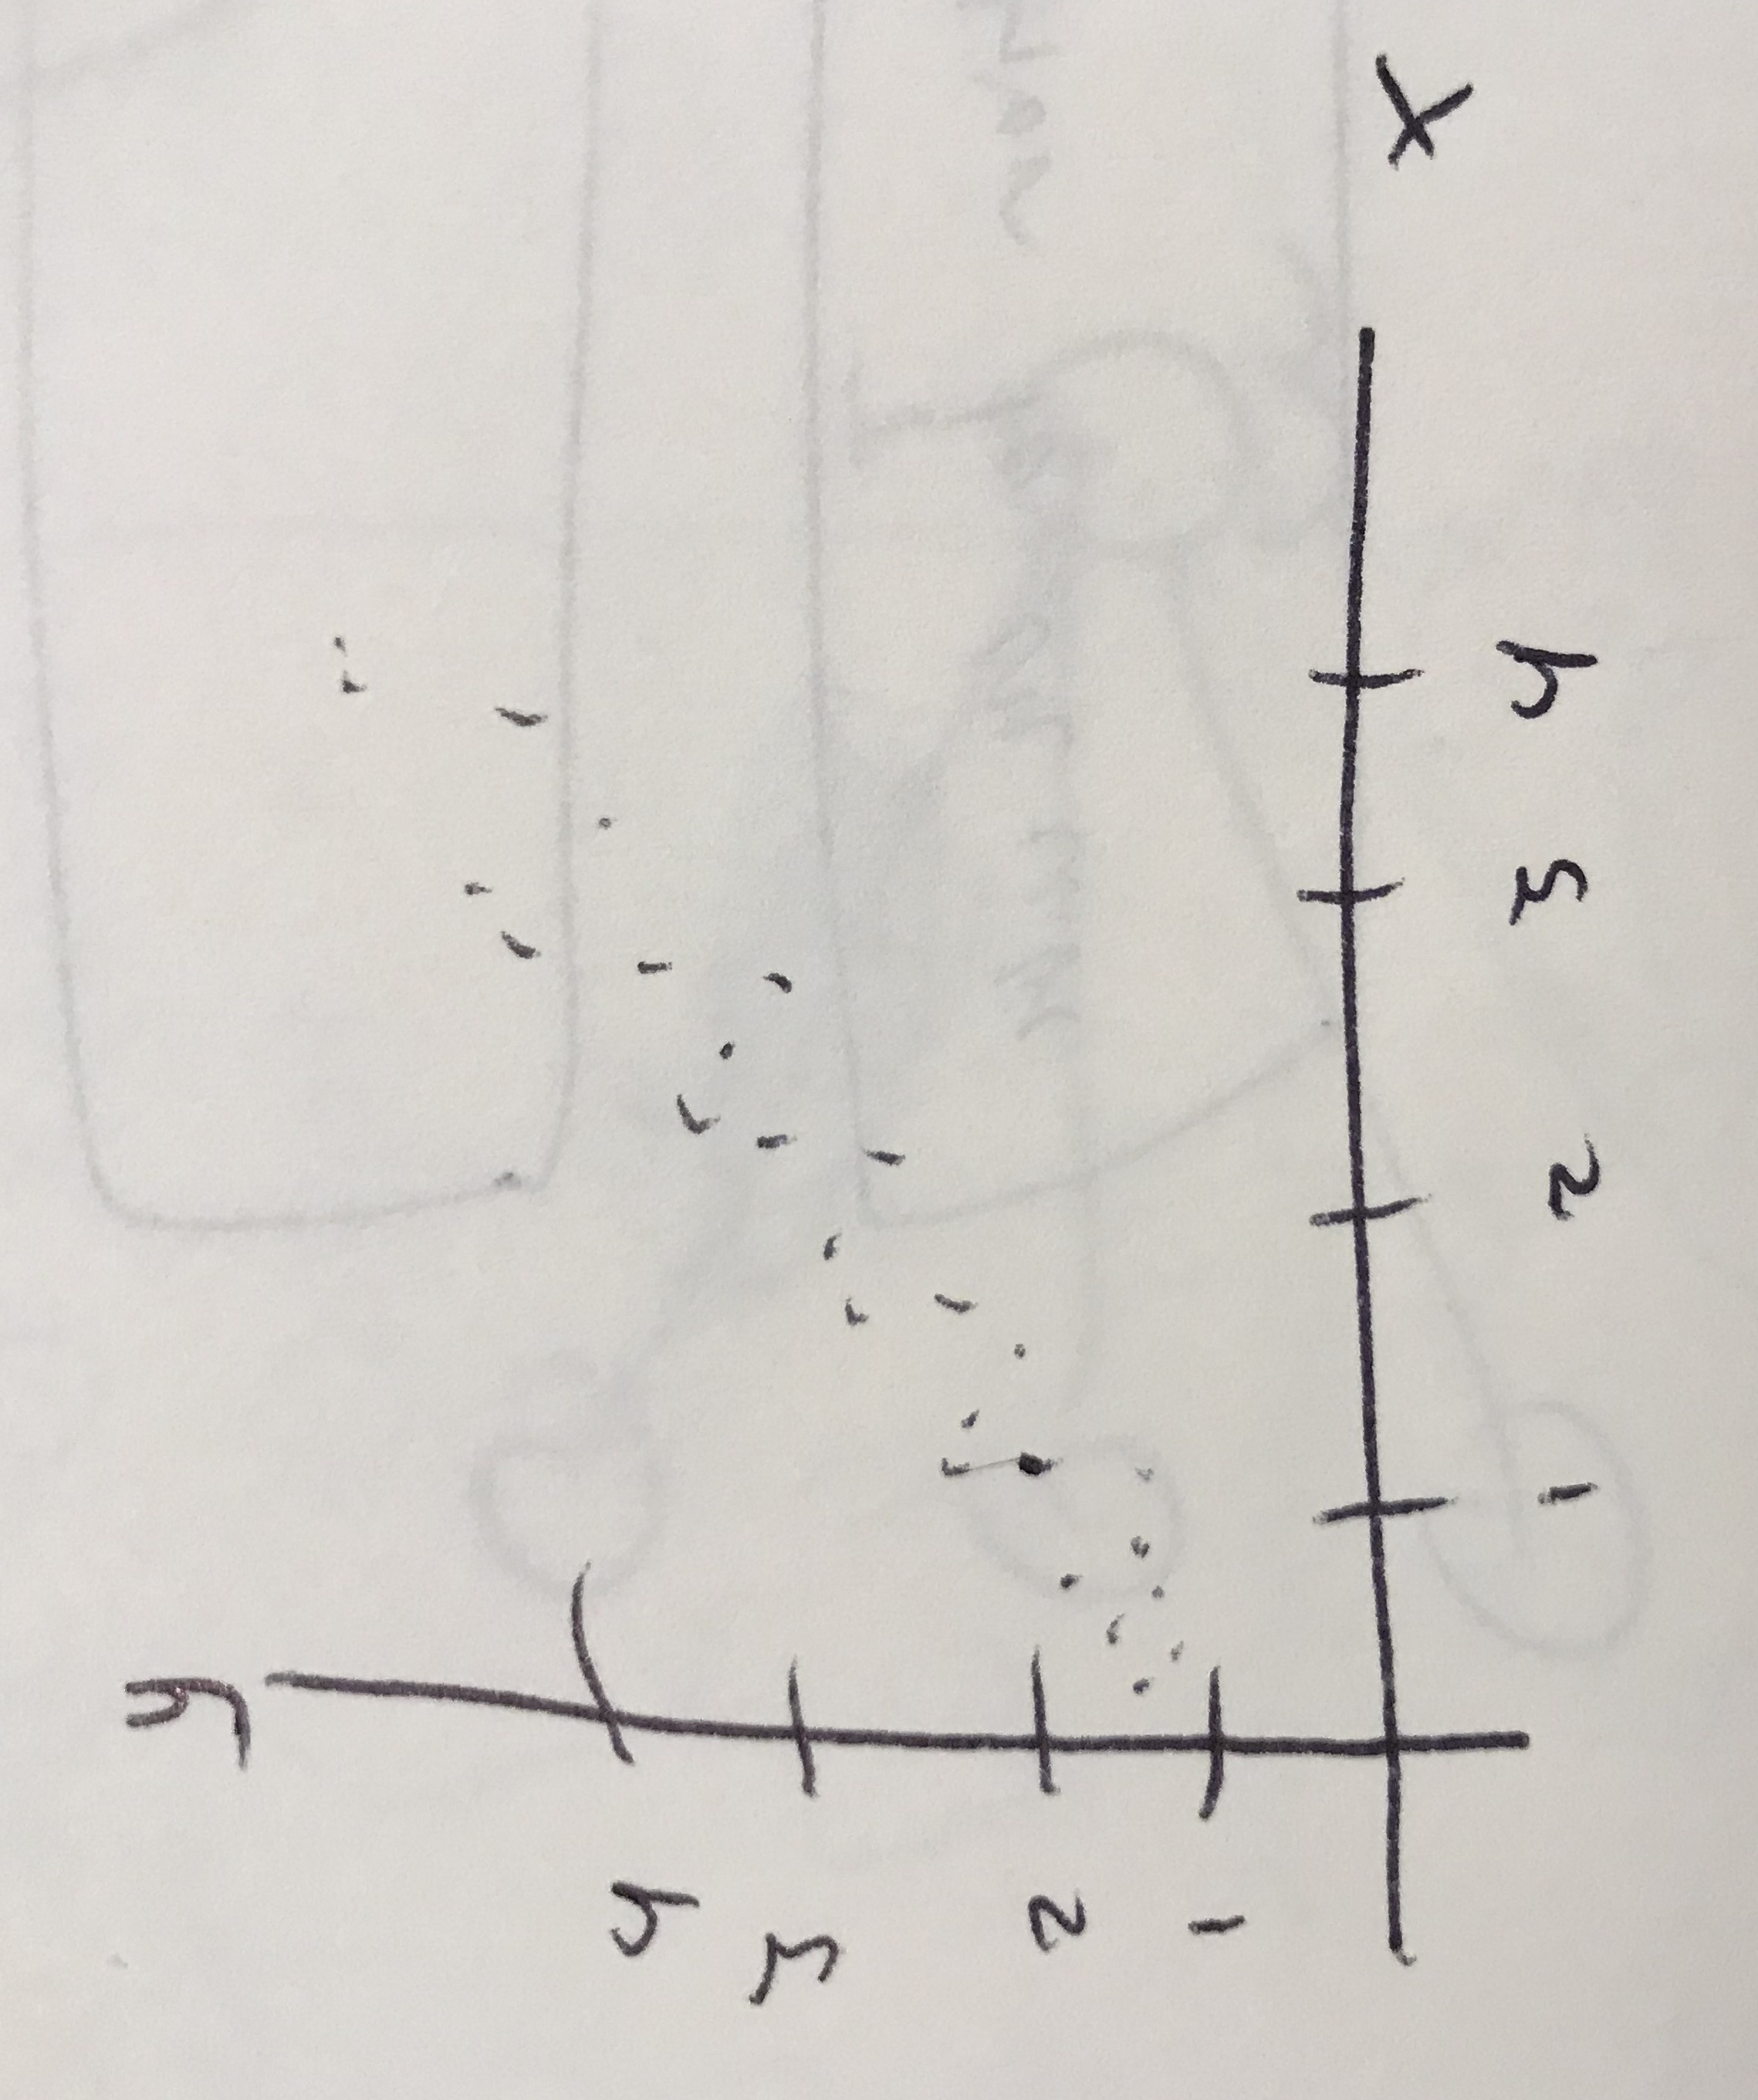
\includegraphics[width=0.5\paperwidth,angle=270]{../LinearRegression/fig/simple_lin_reg.jpg}
    \caption{Data set with clear trend.}
    \label{fig:simple-lin-reg}
\end{figure}

Our eyes are naturally able to detect a very clear trend in this data. If we were to be given a new $\textbf{x}$ data point, how would be predict its target value $y$? We would first fit a line to our data, as in Figure \ref{fig:simple-lin-reg-w-line}:

\begin{figure}[H]
    \centering
    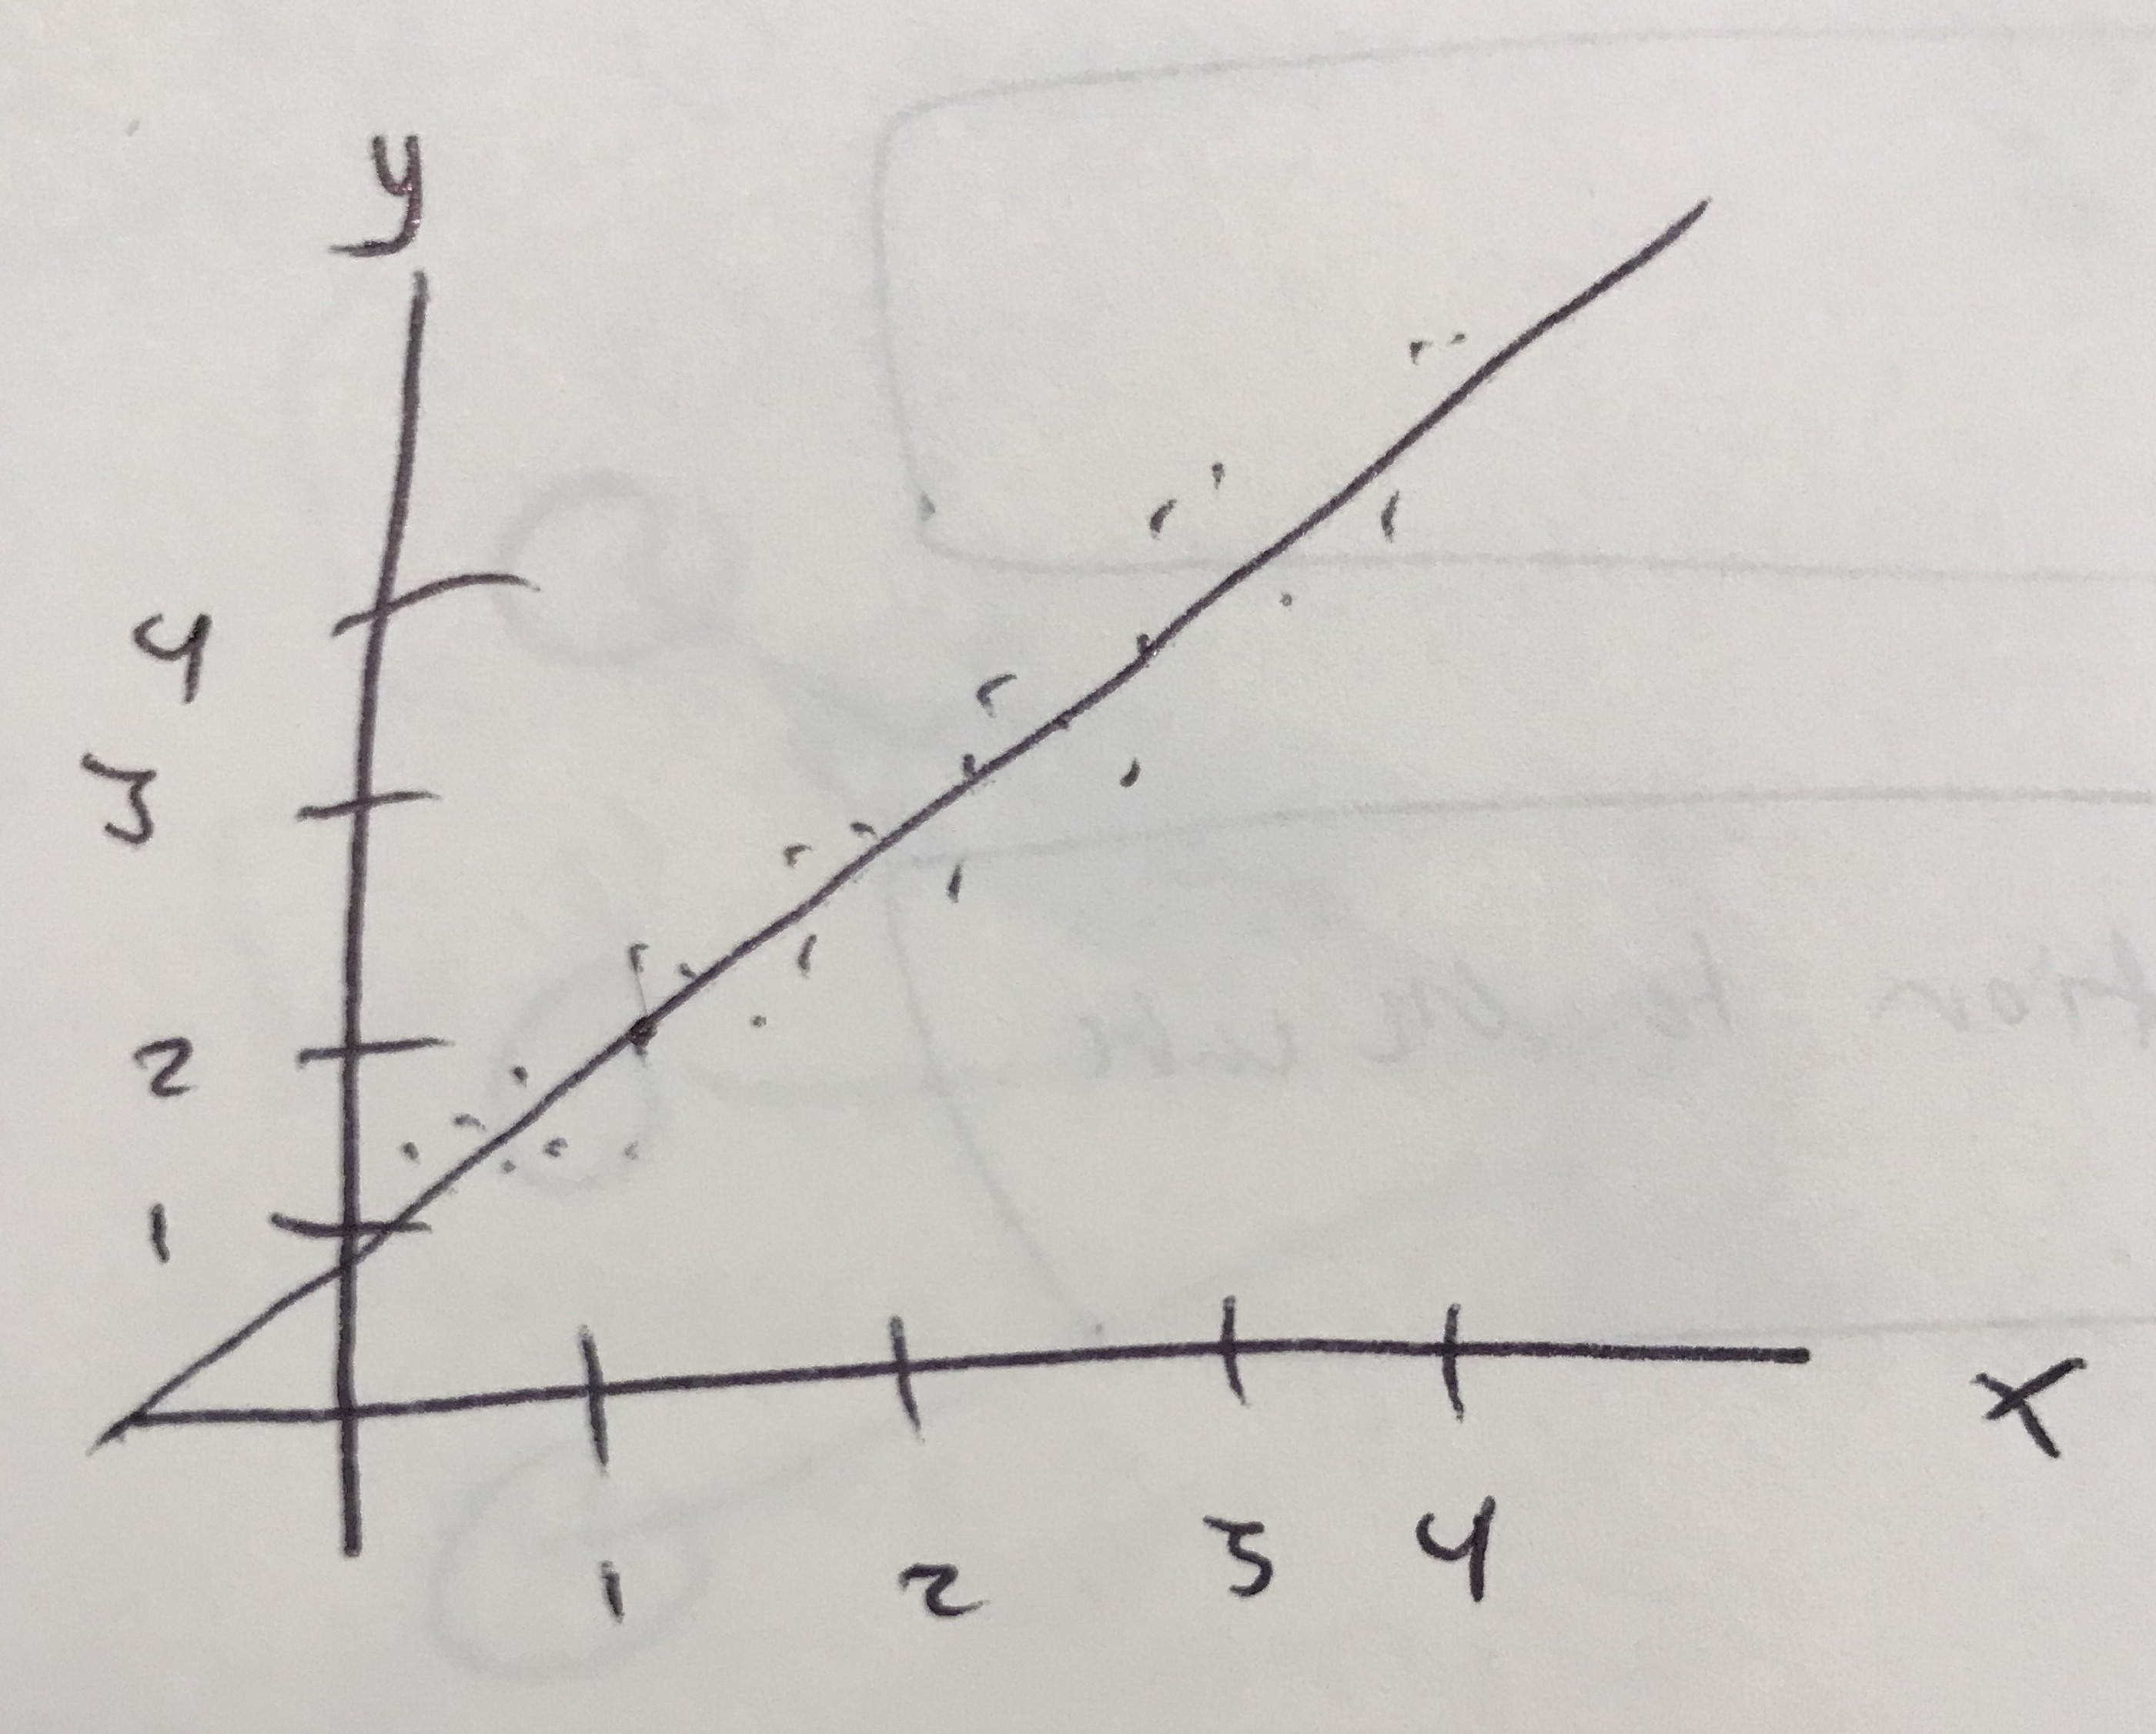
\includegraphics[width=0.5\paperwidth]{../LinearRegression/fig/simple_lin_reg_w_line.jpg}
    \caption{Data set with clear trend, best fitting line included.}
    \label{fig:simple-lin-reg-w-line}
\end{figure}

and then find where on that line the new $\textbf{x}$ value sits.

That is the entirety of linear regression! It fits the `best' line to our data, and then uses that line to make predictions. In 1-D input space, this manifests itself as the simple problem seen above, where we need only find a single bias term $w_{0}$ (which acts as the intercept of the line) and single weight $w_{1}$ (which acts as the slope of the line). However, the same principle applies to higher dimensional data as well. We're always fitting the line (meaning calculate the weights $\textbf{w}$) that give us maximal predictive power.

\readernote{Although our input data points $\textbf{x}$ can take on multiple dimensions, our output data $y$ is always a 1-dimensional real number when dealing with regression problems.}

Now that we have some intuition for what linear regression is, a natural question arises: how do we find these `best' values for $\textbf{w}$? That is the remaining focus of this chapter.

\subsubsection{Finding the Best Fitting Line: Loss}
We can inspect a set of data as presented in **some way to reference the figure above**, and are quite good at fitting a line by hand. When we fit that line, whether we think about it or not, what we're trying to do is make the line as close to all of the data points as possible. We can formalize this notion by introducing the concept of \textbf{loss}, and use it to our advantage in developing a method to automatically fit a line to our data.


\begin{definition}{Loss}{loss}
Loss is the error incurred for a given prediction. It can be thought of as a measurement of difference between the target ($t$) and predicted ($y(\textbf{x}, \textbf{w}$)) values:
\begin{align*}
    \mathcal{L}(\textbf{w}) = \text{target} - \text{prediction} = t - y(\textbf{x}, \textbf{w}) = \boxed{t - \textbf{w}^{T}\textbf{x}}
\end{align*}

Notice that loss is denoted $\mathcal{L}(\textbf{w})$, and it is a function of our parameters $\textbf{w}$, which are used to generate our prediction. Loss can be computed in different manners, and the choice of what loss function to use has important implications that we will discuss.
\end{definition}

Loss is a concept that we will come back to very frequently in the context of supervised machine learning methods.

\subsubsection{Least Squares Loss}
As we mentioned above, there are different methods for computing loss. One of the most commonly used measurements is known as \textbf{Least Squares Loss}. Least squares, as it is often abbreviated, says that the loss for a given data point is the square of the difference between the target and predicted values:

\begin{equation} \label{least-squares-loss-fn}
    \mathcal{L}(\textbf{w}) = (t - \textbf{w}^{T}\textbf{x})^2
\end{equation}

There is a satisfying statistical interpretation for using this loss function which we will explain later in this chapter, but for now it will suffice to discuss some of the properties of this loss function that make it desirable.

First, notice that it will always take on positive values. This is convenient because we can focus exclusively on minimizing our loss, and it also allows us to combine the loss incurred from different data points without worrying about them cancelling out.

A more subtle but enormously important property of this loss function is that we know a lot about how to efficiently optimize quadratic functions. This is not a textbook about optimization, but some quick and dirty intuition that we will take advantage of throughout this book is that we can easily and reliably take the derivative of a quadratic function because they are continuously differentiable. We also know that optima of a quadrative function will be located at points where the derivative of the function is equal to 0, as seen in Figure \ref{fig:quad-deriv-at-2}:

\begin{figure}[H]
    \centering
    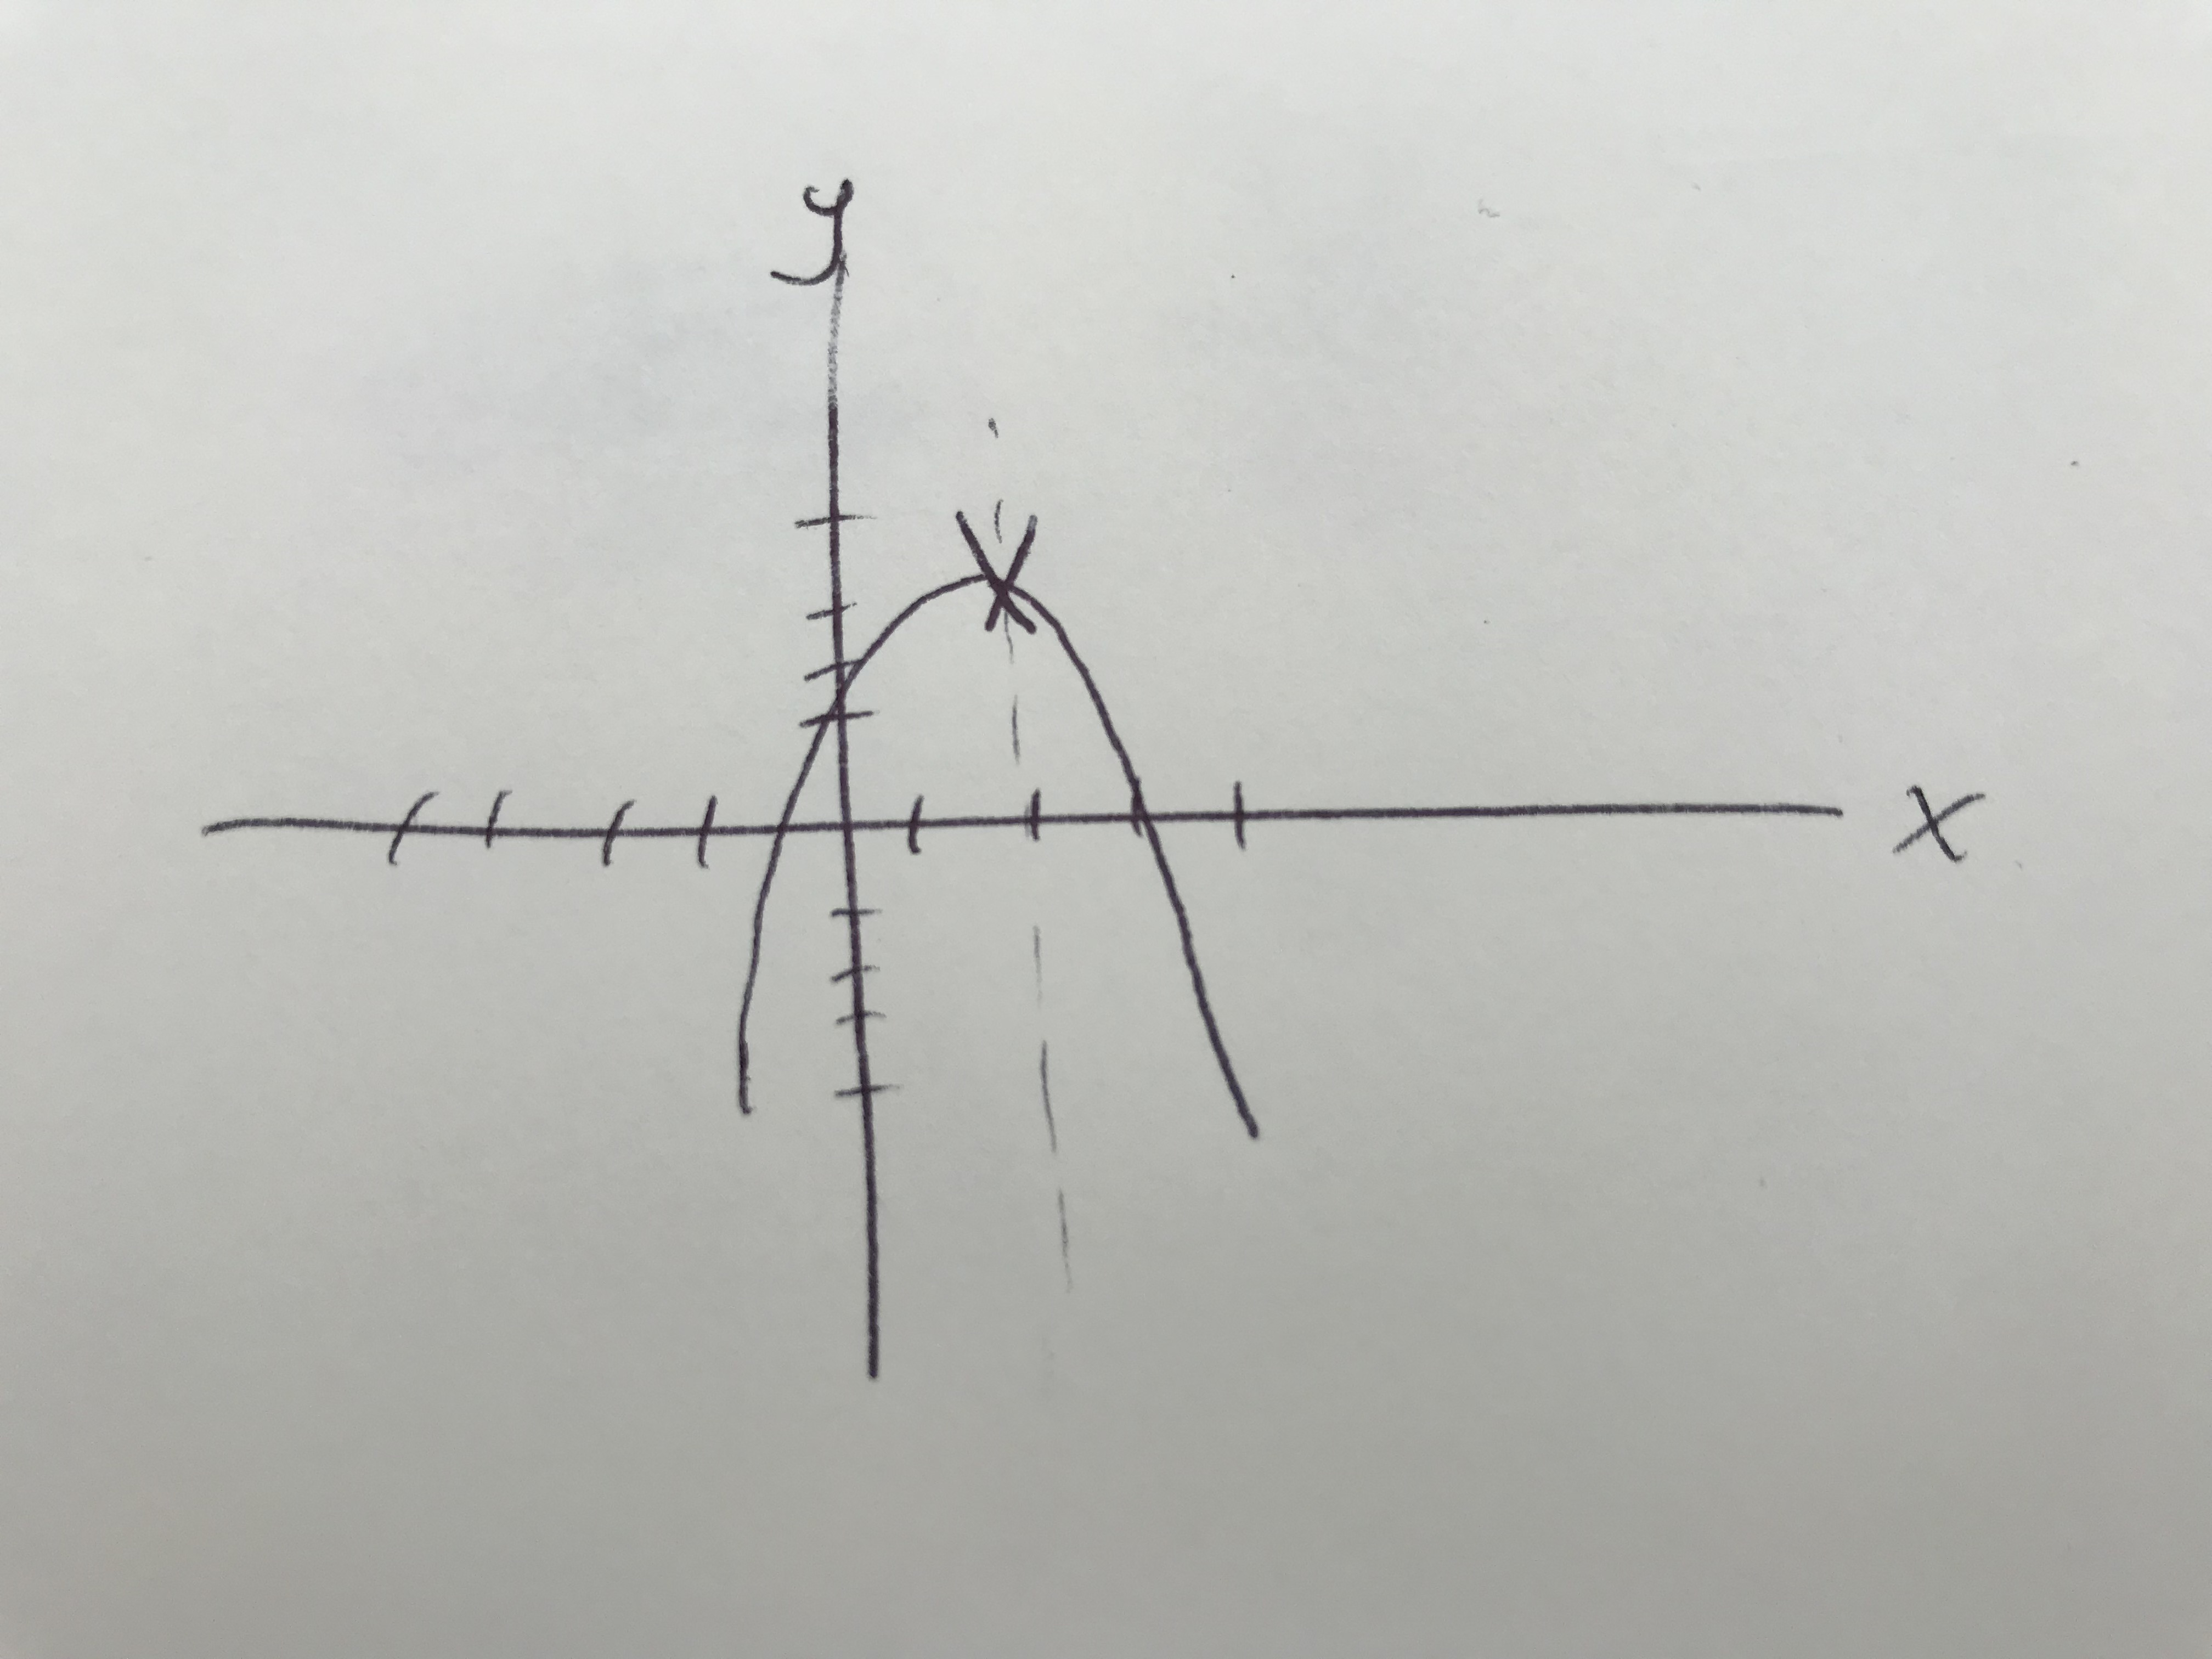
\includegraphics[width=0.5\paperwidth]{../LinearRegression/fig/deriv_at_2.jpg}
    \caption{Quadratic function with clear optimum at $x=2$, where the derivative of the function is 0.}
    \label{fig:quad-deriv-at-2}
\end{figure}

If we compare this to an alternative loss function, such as an absolute value loss:

\begin{align}
    \mathcal{L}(\textbf{w}) = \lvert t - \textbf{w}^{T}\textbf{x} \rvert
\end{align}

We know that this function is not continuously differentiable around its optima, and as a result, it is much less convenient to work with as compared to least squares loss.

** add something about aversion to outliers using least squares loss? **
** add a visualization of what the loss actually looks like for a toy data set (small little red lines from predicted to true) **

\subsubsection{Solving for optimal weights using non-matrix form and matrix form differentiation - MLE solution discussion}
Now that we have our least squares loss function, we can finally begin to fit a line to our data.

First, we can define the loss incurred by parameters $\textbf{w}$ over our entire data set $\textbf{X}$ as follows:

\begin{align}
    \mathcal{L}(\textbf{w}) = \frac{1}{2} \sum_{i=1}^{n} (t - \textbf{w}^{T}\textbf{x})^2
\end{align}

\readernote{Note that we added a constant $\frac{1}{2}$ to the beginning of our loss expression. This scales the loss, which will not change our final result for the optimal parameters. It has the benefit our calculations cleaner once we've taken the gradient of the loss.}

We now want to solve for the values of $\textbf{w}$ that minimize this expression, since a small loss implies that we are doing a good job of predicting values that are close to their true target values.

\begin{derivation}{Least Squares Derivation}{least-squares-derivation}
    We find the optimal weights $\textbf{w}^{*}$ as follows: \\

    Start by taking the gradient of the loss with respect to our parameter $\textbf{w}$:
    \begin{align}
        \nabla \mathcal{L}(\textbf{w}) = \sum_{i=1}^{n} (t - \textbf{w}^{T}\textbf{x})\textbf{x}^{T}
    \end{align}

    Setting this gradient to 0, we have:
    \begin{align}
        0 = \sum_{i=1}^{n} t \textbf{x}^{T} - \textbf{w}^{T} \sum_{i=1}^{n} \textbf{x}\textbf{x}^{T}
    \end{align}

    At this point, it is convenient to rewrite these summations as matrix operations in terms of $\textbf{w}$ instead of $\textbf{w}^{T}$. Note that $(\textbf{w}^{T} \sum_{i=1}^{n} \textbf{x}\textbf{x}^{T})^{T} = \textbf{X}^{T}\textbf{X}\textbf{w}$ and $(\sum_{i=1}^{n} t \textbf{x}^{T})^{T} = \textbf{X}^{T}\textbf{Y}$. Rewriting:
    \begin{align}
        0 = \textbf{X}^{T}\textbf{Y} - \textbf{X}^{T}\textbf{X}\textbf{w}
    \end{align}

    Solving for $\textbf{w}^{*}$:
    \begin{align}
        \textbf{w}^{*} = (\textbf{X}^{T}\textbf{X})^{-1}\textbf{X}^{T}\textbf{Y}
    \end{align}
\end{derivation}

Note that the quantity $(\textbf{X}^{T}\textbf{X})^{-1}\textbf{X}^{T}$ in Derivation \ref{der:least-squares-derivation} has a special name: the \textbf{\textit{Moore-Penrose pseudo inverse}}. You can think of it as a generalization of a matrix inversion operation to a non-square matrix.

\subsubsection{Linear Regression as Projection}
Another common interpretation of linear regression is that of a projection of our targets, $\textbf{Y}$, onto the column space of our inputs $\textbf{X}$. This can be useful for building intuition.

We showed above that the quantity $(\textbf{X}^{T}\textbf{X})^{-1}\textbf{X}^{T}$ can be thought of as the pseudoinverse for our inputs $\textbf{X}$. Let's now consider the case where $\textbf{X}$ is square and the pseudoinverse is equal to the true inverse: $\textbf{X}^{-1} = (\textbf{X}^{T}\textbf{X})^{-1}\textbf{X}^{T}$. We have for our optimal $\textbf{w}^{*}$:
\begin{align*}
    \textbf{w}^{*} = (\textbf{X}^{T}\textbf{X})^{-1}\textbf{X}^{T}\textbf{Y}
\end{align*}
which becomes
\begin{align*}
    \textbf{w}^{*} = \textbf{X}^{-1}\textbf{Y}
\end{align*}
We can recover our target values $\textbf{Y}$ by multiplying either side by $\textbf{X}$:
\begin{align*}
    \textbf{X}\textbf{w}^{*} = \textbf{X}\textbf{X}^{-1}\textbf{Y} \\
    \textbf{X}\textbf{w}^{*} = \textbf{Y}
\end{align*}

We were able to recover our targets $\textbf{Y}$ exactly because $\textbf{X}$ is an invertible tranformation. However, in the general case where $\textbf{X}$ is not invertible and we have to use the approximate pseudoinverse $(\textbf{X}^{T}\textbf{X})^{-1}\textbf{X}^{T}$, we instead recover $\hat{\textbf{Y}}$:
\begin{align*}
    \textbf{X}\textbf{w}^{*} = \textbf{X}(\textbf{X}^{T}\textbf{X})^{-1}\textbf{X}^{T}\textbf{Y} \\
    \textbf{X}\textbf{w}^{*} = \hat{\textbf{Y}}
\end{align*}
where $\hat{\textbf{Y}}$ can be thought of as the closest projection of $\textbf{Y}$ into the column space of $\textbf{X}$. Furthermore, this motivates the intuition that $\textbf{w}^{*}$ is the set of coefficients that best transforms our input space $\textbf{X}$ into our target values $\textbf{Y}$.

\subsubsection{Basis Functions}
There are some situations where our input data $\textbf{X}$ is not the best form of our data for performing linear regression. Because linear regression only scales and combines input variables, it is unable to apply more complex transformations to our data such as a sin or squaring function. In those situations where we need to transform our input variable somehow prior to performing linear regression (which is known as moving our data into a new \textit{basis}, we apply what is known as a \textbf{basis function}.

\begin{definition}{Basis Function}{basis-fn}
    Typically denoted by the symbol $\phi(\cdot)$, a basis function is a transformation applied to an input data point $\textbf{x}$ to move our data into a different \textit{input basis}, which is another phrase for \textit{input domain}. \\

    For example, consider our original data point:
    \begin{align*}
        \textbf{x} = (x_{1}, x_{2})'
    \end{align*}
    We may choose our basis function $\phi(\textbf{x})$ such that our transformed data point in its new basis is:
    \begin{align*}
        \textbf{x} = (x_{1}, x_{1}^2, x_{2}, \sin{x_{2}})'
    \end{align*}

    Using a basis function is so common that we will sometimes describe our input data points as $\boldsymbol{\phi} = (\phi_{1}, \phi_{2}, ..., \phi_{D})'$.
\end{definition}

Basis functions are very general - they could specify that we just keep our input data the same. As a result, it's common to rewrite the least squares loss function from Equation \ref{least-squares-loss-fn} for linear regression in terms of the basis function applied to our input data:

\begin{equation} \label{least-squares-loss-fn-w-basis}
    \mathcal{L}(\textbf{w}) = \frac{1}{2} \sum_{i=1}^{n} (t - \textbf{w}^{T}\boldsymbol{\phi})^2
\end{equation}

To motivate why we might need basis functions for performing linear regression, let's consider this graph of 1-dimensional inputs \textbf{X} along with their target outputs \textbf{Y}:

\begin{figure}[H]
    \centering
    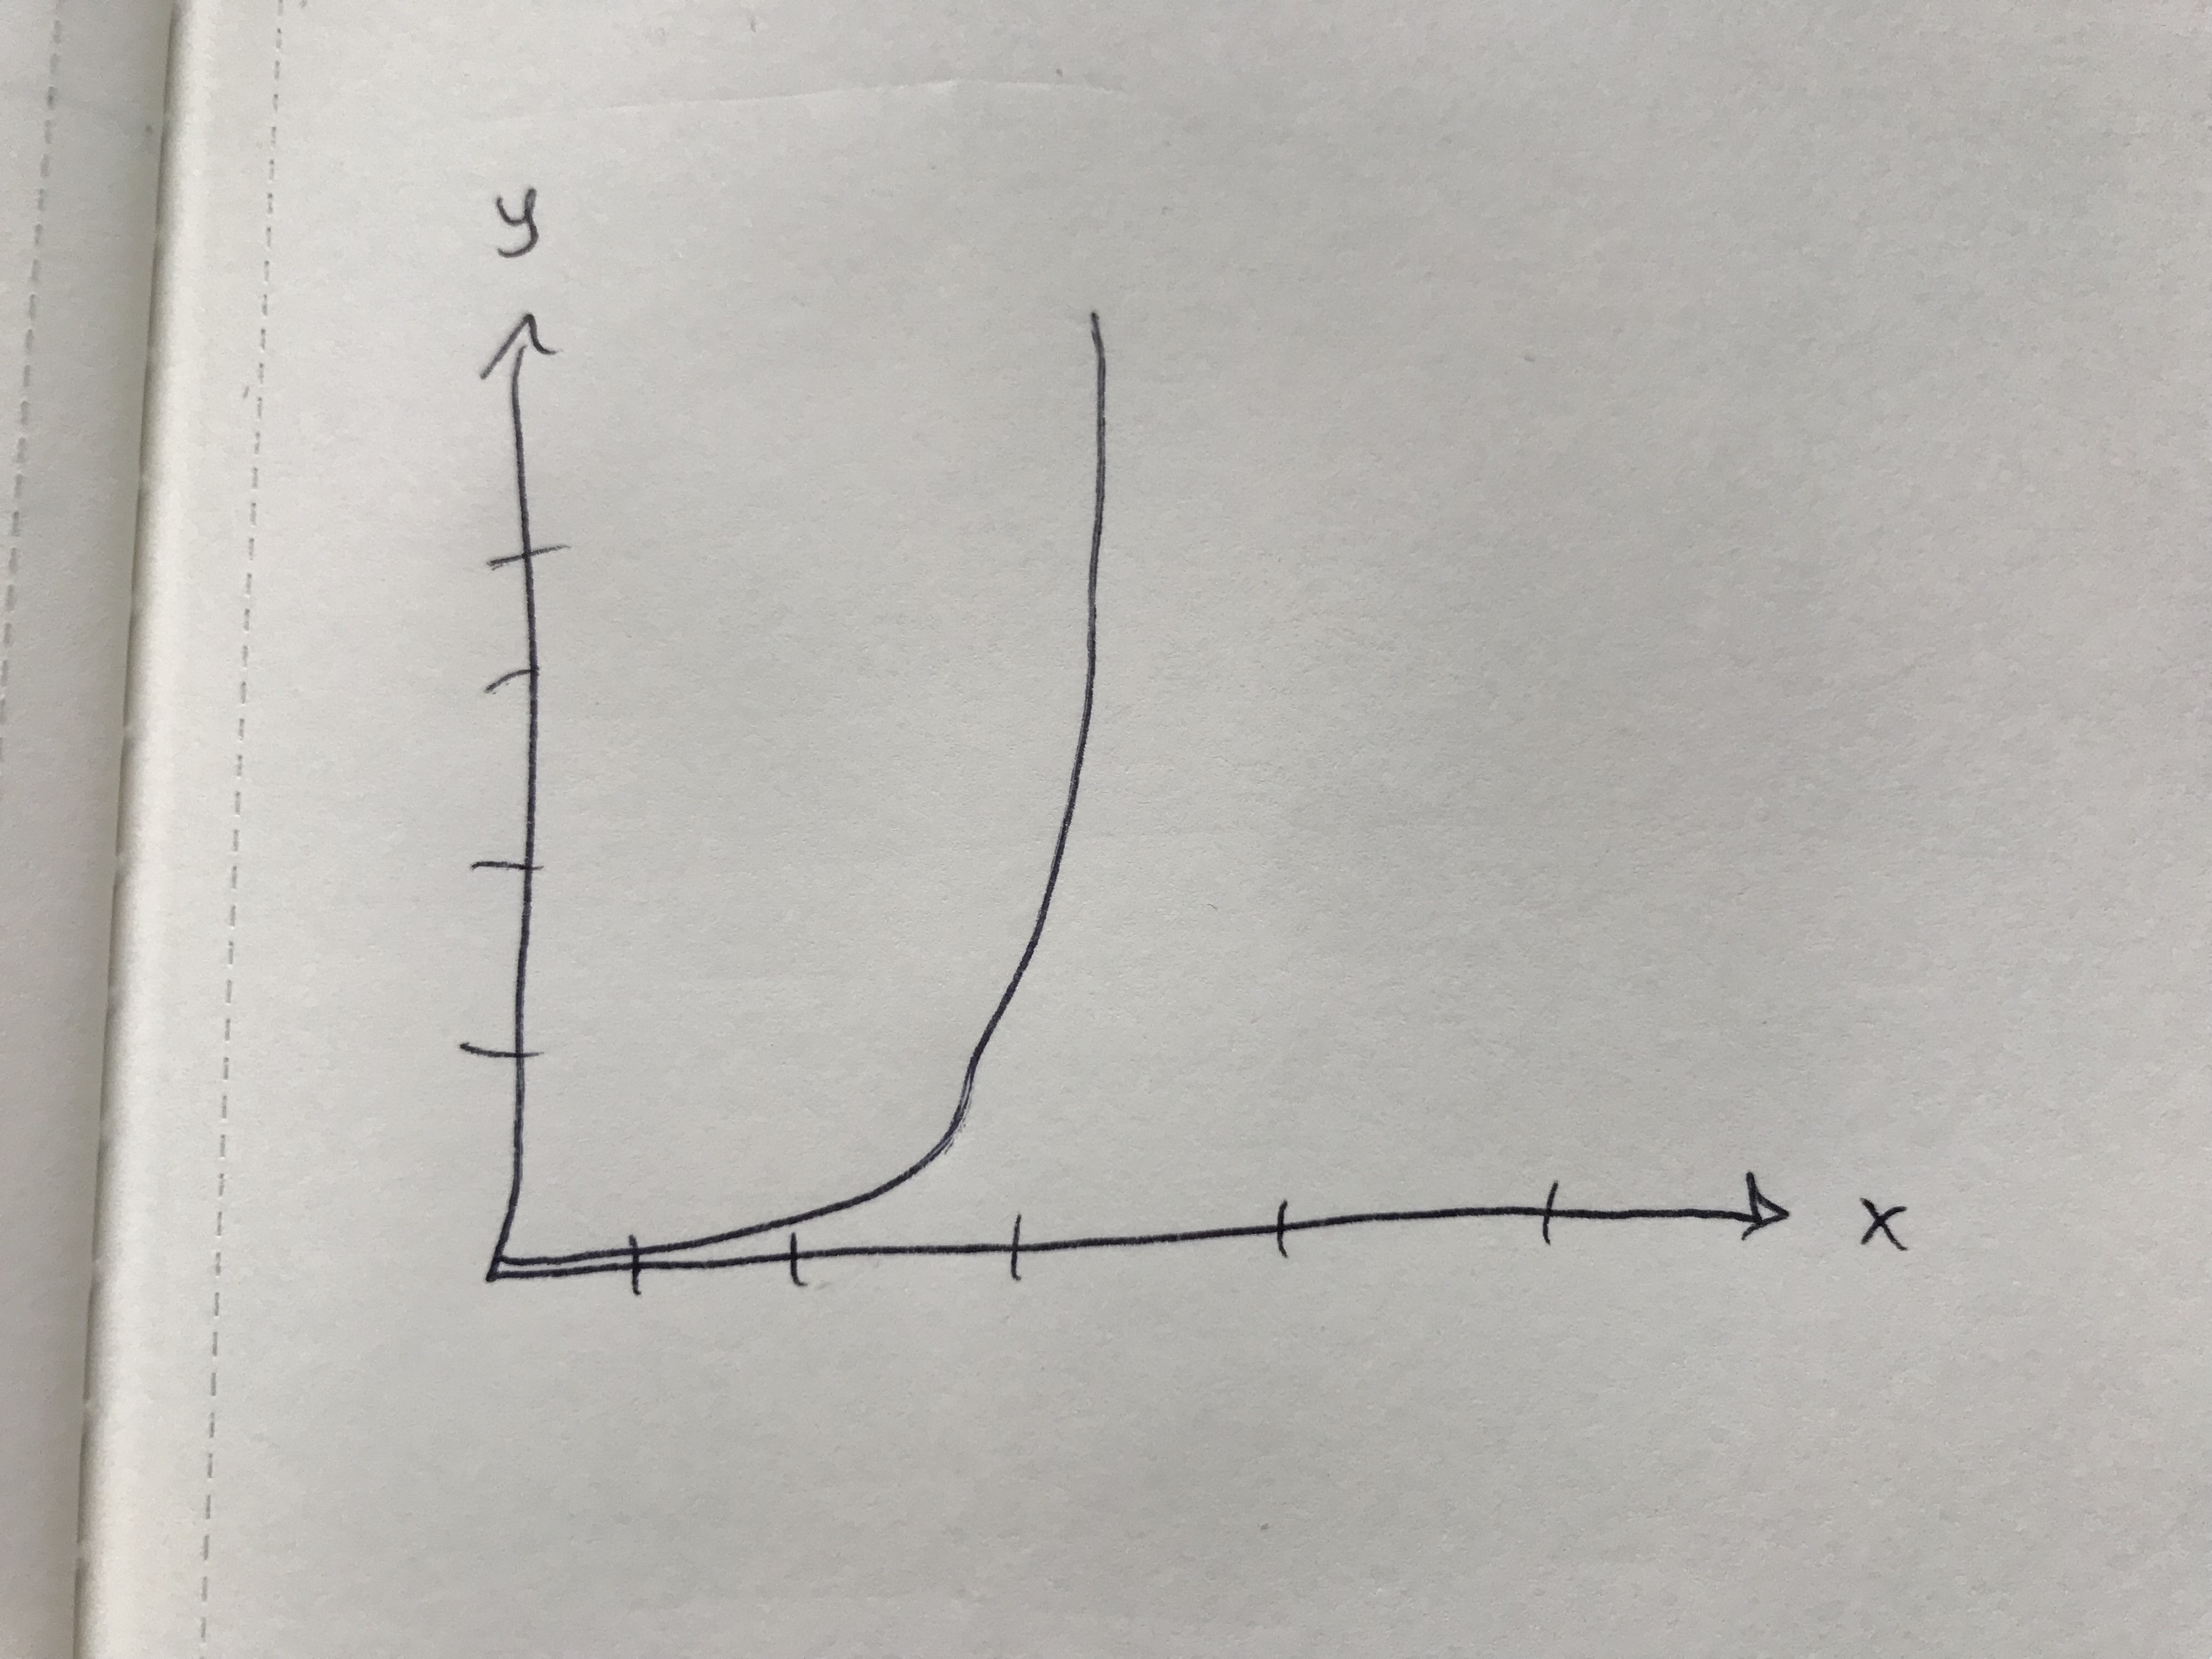
\includegraphics[width=0.5\paperwidth]{../LinearRegression/fig/lin_reg_no_basis_fn.jpg}
    \caption{Data with no basis function applied.}
    \label{fig:lin-reg-no-basis-fn}
\end{figure}

As we can see, we're not going to be able to fit a good line to this data. The best we can hope to do is something like this:

\begin{figure}[H]
    \centering
    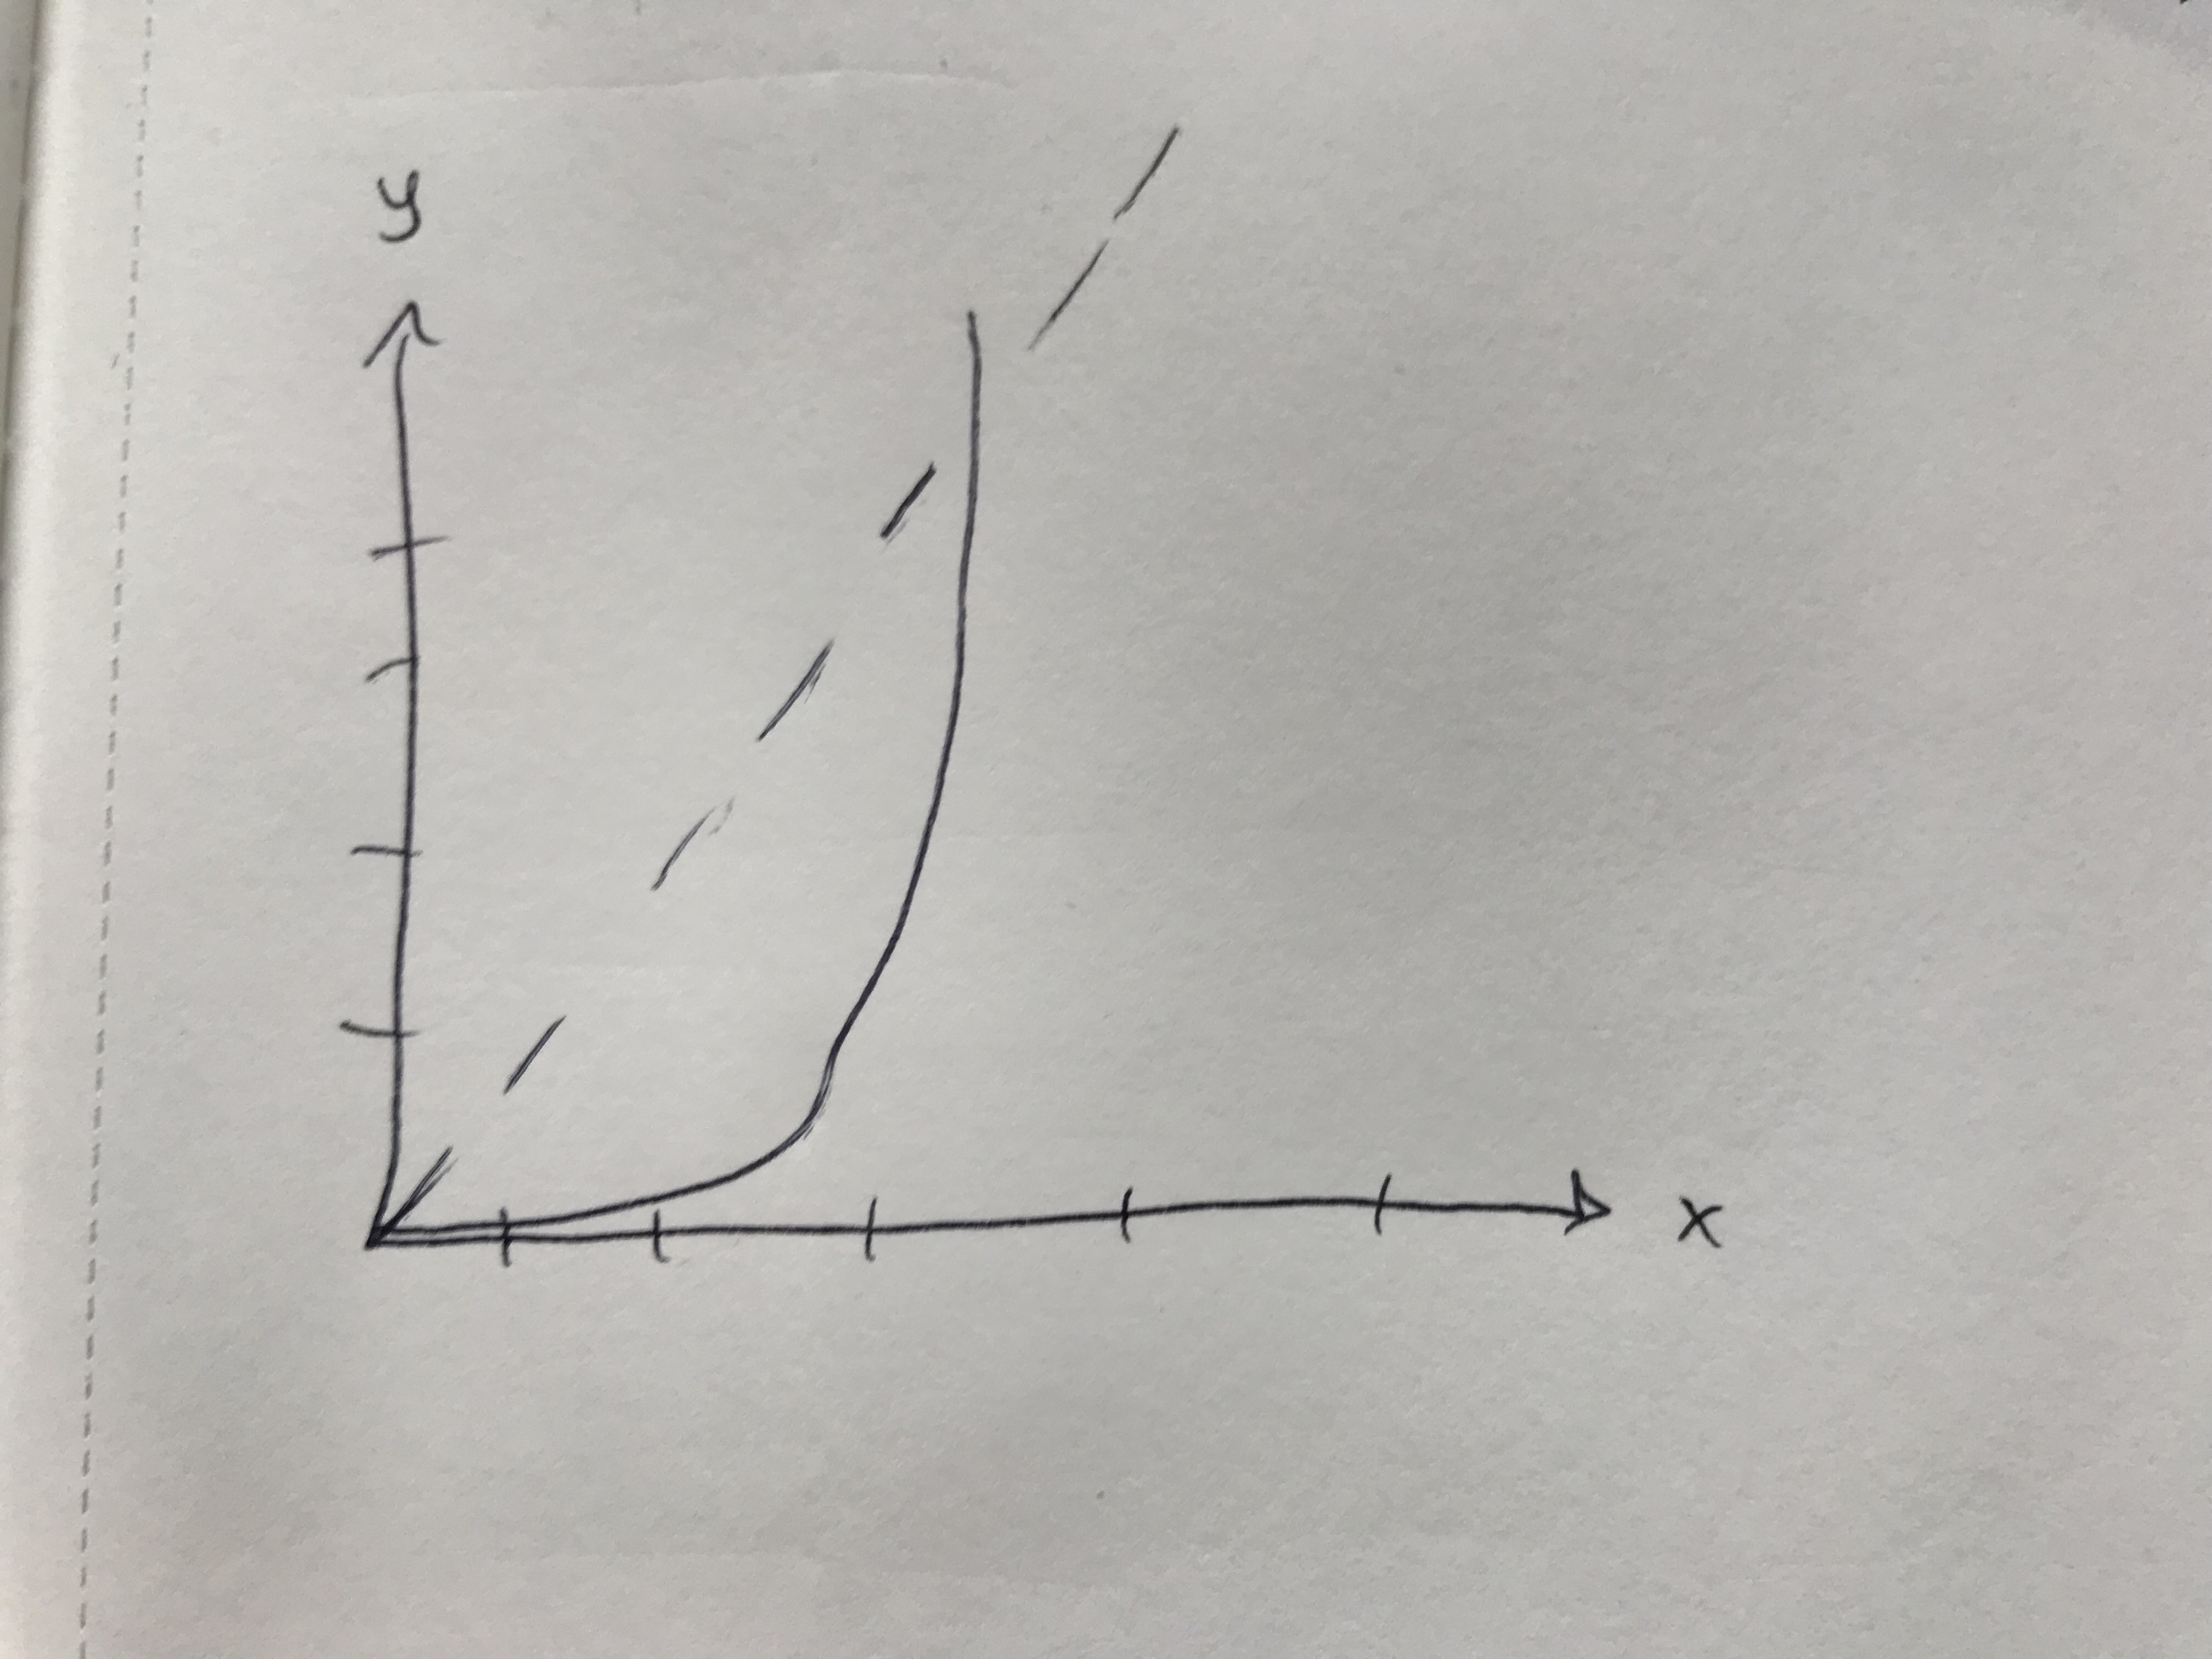
\includegraphics[width=0.5\paperwidth]{../LinearRegression/fig/lin_reg_no_basis_fn_fitted.jpg}
    \caption{Data with no basis function applied, attempt to fit a line.}
    \label{fig:lin-reg-no-basis-fn-fitted}
\end{figure}

However, if we just apply a simple basis function to our data, in this case the simple square root function, $\phi(\textbf{x}) = (\sqrt{x_{1}})'$, we now have this data:

\begin{figure}[H]
    \centering
    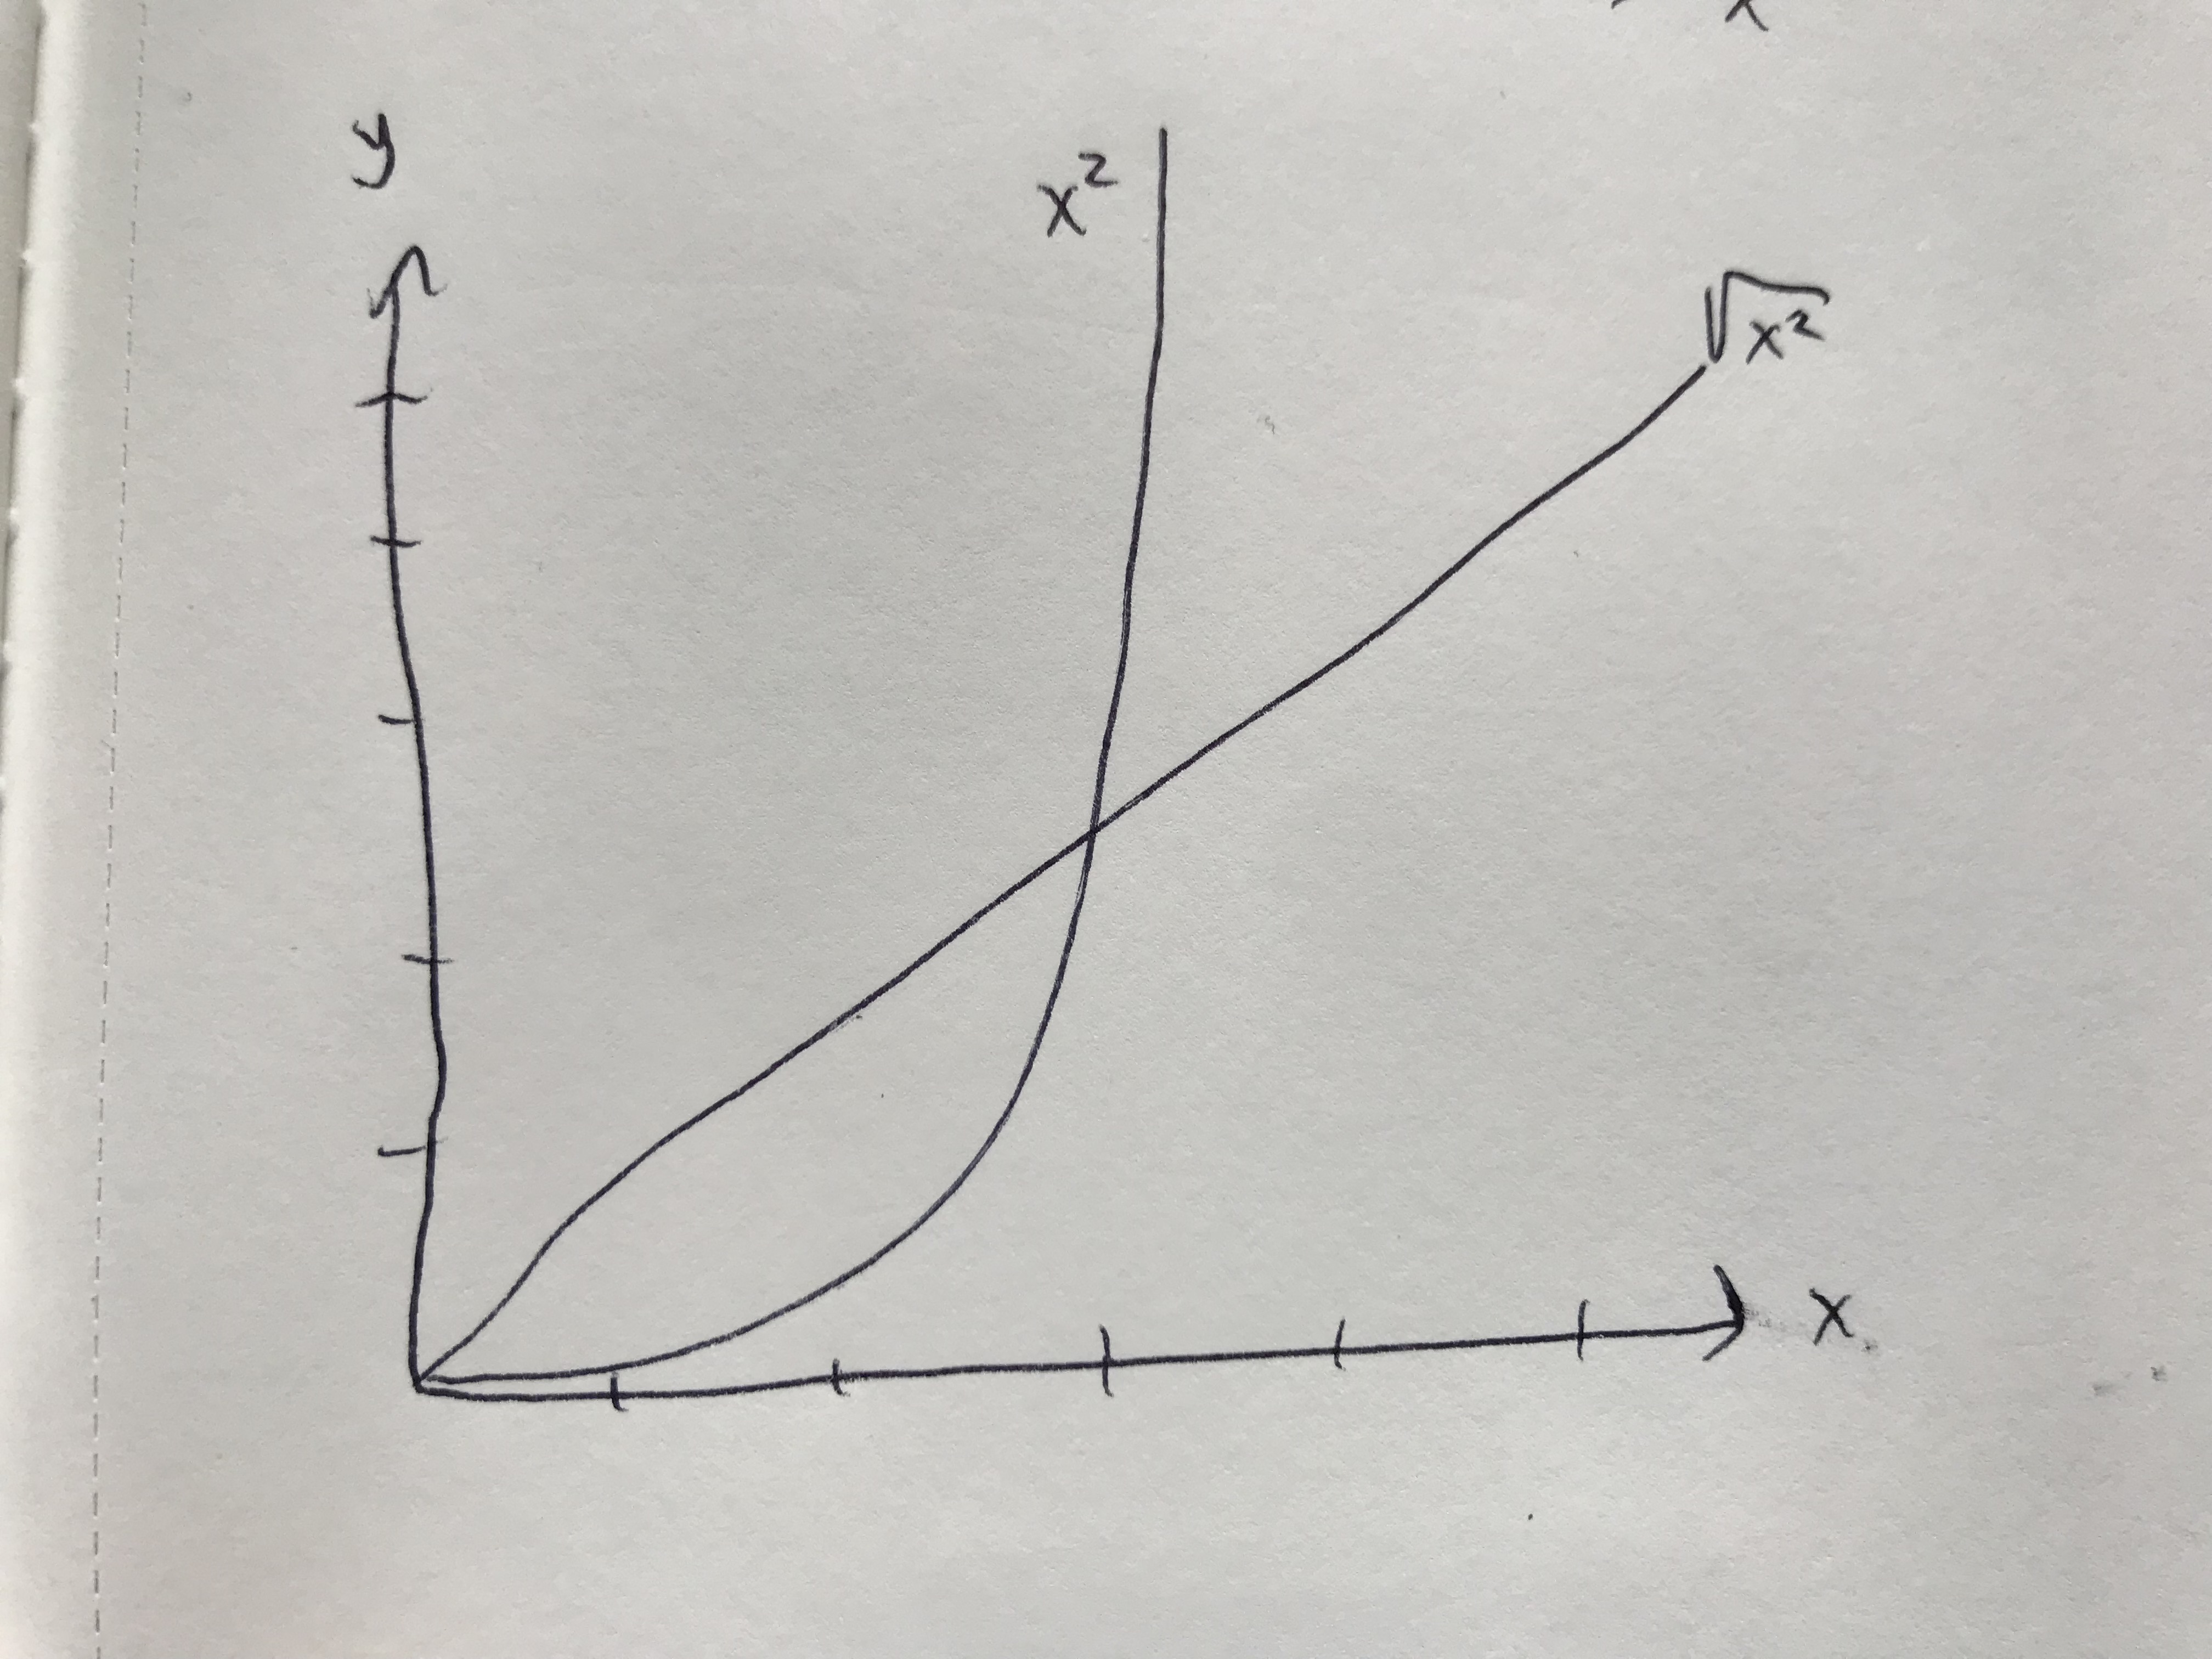
\includegraphics[width=0.5\paperwidth]{../LinearRegression/fig/lin_reg_w_basis_fn.jpg}
    \caption{Data with square root basis function applied.}
    \label{fig:lin-reg-w-basis-fn-fitted}
\end{figure}

We now see that we can fit a very good line to our data, thanks to basis functions. Still, the logical question remains: how can I choose the appropriate basis function? This toy example had a very obviously good basis function, but in general with high dimensional, messy input data, how do we choose the basis function we need?

The answer is that this is not an easy problem to solve. Often, you may have some domain specific knowledge that tells you to try a certain basis, such as if you're working with chemical data and know that an important equation involves a certain function of one of your inputs. However, more often than not we won't have this expert knowledge either. Later on, we will discuss methods for discovering the best basis functions for our data automatically.

\subsubsection{Regularization}
How we can mitigate the problem of overfitting, especially if we want to try a lot of basis functions
why we need it, different types, what its effects are
Now that we've introduced the idea of basis functions, you might wonder why we don't just try adding many basis transformations to our input data to find a good transformation. For example, we might use this large basis function:

\begin{align*}
    \phi(\textbf{x}) = (x_{1}, x_{1}^{2}, ..., x_{1}^{100}, x_{2}, x_{2}^{2}, ..., x_{2}^{100}, x_{D}, x_{D}^{2}, ..., x_{D}^{100})'
\end{align*}

all we've done is tried transforming every input data point up to 100 degrees. Can you imagine what might happen now that we've done this?

Let's say our input data point \textbf{x} is simply 1-dimensional, and we apply the basis function described above, so that after the transformation each data point is represented by 100 values. Say we have 100 data points on which to perform linear regression, and because our transformed input space has 100 values, we have 100 parameters to fit. In this case, with one parameter per data point, it's possible for us to fit our regression line perfectly to our data so that we have 0 loss! But is this a desirable outcome? The answer is no, and we'll provide a visual example to illustrate that.

Imagine this is our data set. There is a very clear trend in this data, and you would likely draw a line that looks something like this to fit it:
** image of nicely fitted line **

However, imagine now we performed a large basis transformation like tha one described above. If we do that, it's possible for us to fit our line perfectly, threading every data point, just like this:
** threaded line image **

Let's see how both of these would perform on new data points. With our first regression line, if we have a new data point $\textbf{x} = (1)'$, we would predict a target value of \textit{something}, which most people would agree is a pretty good measurement. However, with the second regression line, we would predict a value of \textit{something else}, which most people would agree does not describe the general trend in the data. So how can we handle this problem elegantly?

Examining our loss function in Equation \ref{least-squares-loss-fn-w-basis}, we see that right now we're only penalizing predictions that are not correct. Intuitively, if we wanted to avoid this problem of a convoluted line, we should also penalize the total size of our weights \textbf{w}. The effect of this is to discourage lots of complex weight values that produce a messy regression line. Instead, by penalizing large weights, we favor simple regression lines like the one in ** figure of simple line that we drew ** that take advantage of only the most important basis functions.

The concept that we are introducing, penalizing large weights, is what is known as \textbf{regularization}, and it's one that we will see come up often in different machine learning methods.

\begin{definition}{Regularization}{regularization}
    The idea of adding a loss for large weight values, which encourages simple solutions that take advantage of the most important information from our data.
\end{definition}

There is obviously a tradeoff between how aggressively we regularize our weights, and we will formalize this tradeoff in the next section. However, for now, we will simply introduce a regularization parameter $\lambda$, to our least squares loss function:

\begin{equation} \label{least-squares-loss-fn-w-regularization}
    \mathcal{L}(\textbf{w}) = \frac{1}{2} \sum_{i=1}^{n} (t - \textbf{w}^{T}\boldsymbol{\phi})^2 + \lambda\textbf{w}^{2}
\end{equation}

The effect of $\lambda$ is to penalize large weight parameters. The larger $\lambda$ is, the more we will favor simple solutions. In the limit $\lim_{\lambda\to\infty} \mathcal{L}(\textbf{w})$, we will drive all weights to 0, while with a nonexistant $\lambda = 0$ we will apply no regularization at all. Notice that we're squaring our weight parameters - this is known as \textit{L2 norm regularization} or \textit{ridge regression}. We will discuss the different types of regularization later on, but for now just know that L2 norm regularization is very common.

To build some intuition about this regularization parameter, let's see how different values of it will produce different regression lines:

** three graphs at different regularization levels **

Notice how larger values of $\lambda$ produce less complex lines, which is the effect of applying more regularization. This is very nice for the problem we started with - which was wanting a way to choose which basis functions we wanted to use. With regularization, we can select many basis functions, and then allow regularization to `prune' the ones that aren't meaningful (by driving their weight parameters to 0). While this doesn't mean that we should use as many basis transformations as possible (there will be computational overhead for doing this), it does allow us to create a much more flexible linear regression model without creating a convoluted regression line.

\subsubsection{Bias-Variance Tradeoff and Decomposition}
Now that you know about regularization, you might have some intuition about why we want to keep a simple line instead of a complex line. A complex line, while it might fit all of our data, potentially does worse on new incoming data. On the other hand, a line that is too simple might not vary enough to provide good predictions at all. This is a very common pattern in machine learning, and it's known as the \textbf{bias-variance tradeoff}.

The phenomenon we encountered in the previous section is not unque ot linear regression. So we have a problem here: on the one hand we don't know the basis we would like to transform our data into, but on the other hand we don't want to end up in this situation where we fit a convoluted line that doesn't generalize well to future data points. This phenomenon is not unique to linear regression- it's actually a very fundamental concept in machine learning that's known as the \textbf{bias-variance tradeoff}.

\begin{definition}{Bias-Variance Tradeoff}{bias-variance-tradeoff}
    When construction machine learning models, we have a choice between fitting very tightly to our training data (high variance, low bias), ... todo
\end{definition}



\subsubsection{explanation and derivation of bias-variance decomposition}
\subsubsection{cross-validation as a means of inspecting model performance}
\subsubsection{connect least squares loss for linear regression to bayesian linear regression}
\subsubsection{ridge regression as adding zero response data, sequential estimation, different types of regularization}
\subsubsection{predictive distribution}